\chapter{Campos gravitacionales d'ebiles y ondas gravitacionales}\label{capdebil1}

\section{Expansi'on en potencias de \texorpdfstring{$G$}{G}}
Las ecuaciones de Einstein son no-lineales en la m'etrica. Por esto, sus
soluciones dependen de forma nolineal del tensor de energ'ia-momentum de la
materia (que asumimos conocido). Como $T^{\mu\nu}$ aparece al lado derecho de las ecuaciones de Einstein siempre multiplicado por la constante de gravitaci'on $G$, es decir, en la combinaci'on $GT^{\mu\nu}$, entonces las componentes m'etricas depender'an no-linealmente de $G$. Podemos verificar esta propiedad, por ejemplo, en el caso de la soluci'on de Schwarzschild.

Asumiendo que el \textit{campo gravitacional es d'ebil} (curvatura peque\~na), pero \textit{no necesariamente estacionario}, es posible desarrollar un \textit{m'etodo perturbativo}
para expresar las soluciones de las ecuaciones de Einstein como una serie de
t'erminos, cada uno proporcional a una potencia dada de la constante de gravitaci'on $G$.

%Aqu'i consideraremos s'olo la aproximaci'on a primer orden.
% Adem'as las velocidades de
% las part'iculas no necesitan ser peque\~nas comparadas con la velocidad de la
% luz.

Dividimos la m'etrica en
\begin{equation} \label{exp01}
g_{\mu\nu}=\eta_{\mu\nu}+h_{\mu\nu}, \qquad \left|h_{\mu\nu}\right|<< 1,
\end{equation}
donde $\eta$ es la m'etrica plana, es decir, $Riemann(\eta)=0$ y usaremos
coordenadas ``cuasi-inerciales'' $x^\mu$ tales
que $\eta_{\mu\nu}=diag(+1,-1,-1,-1)$. Adem'as, separaremos la perturbaci'on $h_{\mu\nu}$ en una serie de potencias de $G$, de modo que
\begin{equation}
h_{\mu\nu}=h^{(1)}_{\mu\nu}+h^{(2)}_{\mu\nu}+h^{(3)}_{\mu\nu}+\cdots,
\end{equation}
donde $h^{(n)}_{\mu\nu}$, $n=0,1,\cdots$, denota el t'ermino proporcional a $G^n$. En particular $h^{(0)}_{\mu\nu}=\eta_{\mu\nu}$.

%Nos concentraremos en el t'ermino de primer orden, de modo que
% consideraremos que $h_{\mu\nu}$ es lineal en $G$, lo que denotamos por
% $h=O(G)$.

% Recuerde que en el sistema solar
% $\left|h_{\mu\nu}\right|\sim \frac{|\phi|}{c^2} \sim
% \frac{GM_\odot}{c^2R_\odot} \sim 10^{-6}$.

Realizaremos una expansi'on similar para cada cantidad relevante. Por ejemplo,
\begin{align}
\Gamma^\lambda_{\mu\nu} &= \Gamma^{\lambda}_{(1)\mu\nu}+\Gamma^{\lambda}_{(2)\mu\nu}+\Gamma^{\lambda}_{(3)\mu\nu}+\cdots, \\
R_{\mu\nu} &= R^{(1)}_{\mu\nu}+R^{(2)}_{\mu\nu}+R^{(3)}_{\mu\nu}+\cdots,\\
G_{\mu\nu} &= G^{(1)}_{\mu\nu}+G^{(2)}_{\mu\nu}+G^{(3)}_{\mu\nu}+\cdots.
\end{align}
Note que, ya que el t'ermino de orden cero es la m'etrica plana (y adem'as usamos coordenadas donde esta m'etrica plana es constante), las expansiones de la conexi'on, curvatura, y el tensor de Einstein comienzan con el orden 1.

Similarmente, es necesario en general considerar una expansi'on del tensor de energ'ia-momentum de la materia:
\begin{equation}
T_{\mu\nu}=T^{(0)}_{\mu\nu}+T^{(1)}_{\mu\nu}+T^{(2)}_{\mu\nu}+\cdots.
\end{equation}
Aqu'i $T_{\mu\nu}^{(0)}$ representa el tensor de energ'ia-momentum de la materia a orden cero en $G$, \textbf{como si la materia estuviese distribuida en un espacio plano}. Recuerde que en general $T_{\mu\nu}$ depende de la m'etrica\footnote{Por ejemplo, para un fluido perfecto $T^{\mu\nu}=(\rho+p/c^2) u^\mu u^\nu-p\,g^{\mu\nu}$.}, por lo que es necesario realizar la expansi'on correspondiente para $T_{\mu\nu}$.

Con esto, las ecuaciones de Einstein adoptan la forma
\begin{equation}
G^{(1)}_{\mu\nu}+G^{(2)}_{\mu\nu}+G^{(3)}_{\mu\nu}+\cdots=
\frac{8\pi G}{c^4}\left(T^{(0)}_{\mu\nu}+T^{(1)}_{\mu\nu}+T^{(2)}_{\mu\nu}+\cdots\right),
\end{equation}
que \textit{separaremos}, consistentemente, en
\begin{align}
G^{(1)}_{\mu\nu}&=\frac{8\pi G}{c^4}T^{(0)}_{\mu\nu},\label{orden1}\\
G^{(2)}_{\mu\nu}&=\frac{8\pi G}{c^4}T^{(1)}_{\mu\nu},\\
G^{(3)}_{\mu\nu}&=\frac{8\pi G}{c^4}T^{(2)}_{\mu\nu}\label{orden3},
\end{align}
etc.

\subsection{Expansi'on a primer orden}
\subsubsection{M'etrica}

Primero requerimos calcular la m'etrica inversa $g^{\mu\nu}$
\begin{equation}
g^{\mu\nu}=\eta^{\mu\nu}+g^{\mu\nu}_{(1)}+g^{\mu\nu}_{(2)}+\mathcal{O}(G^3).
\end{equation}
Un c'alculo simple muestra que
\begin{align}
g^{\mu\nu}_{(1)}&=-\eta^{\mu\lambda}\eta^{\nu\rho}h_{\lambda\rho}=:-h^{\mu\nu}_{(1)} .
\end{align}

\textit{Por convenci'on, en el contexto de la expansi'on realizada subimos y bajamos los 'indices usando la m'etrica plana} $\eta$. As'i, por ejemplo, $h^{(1)}:=h^\mu_{(1)}{}_\mu=\eta^{\mu\nu}h^{(1)}_{\mu\nu}$ es la \textit{traza} del tensor $h^{(1)}_{\mu\nu}$ y $\square :=\partial_\mu\partial^\mu=\eta^{\mu\nu}\partial_\mu\partial_\nu$ es el operador de onda.
\subsubsection{Conexi'on}\label{sec:conG1}

La primera contribuci'on a los s'imbolos de Christoffel resultan ser
\begin{align}
\Gamma^\lambda_{(1)\mu\nu}&=\frac{1}2\eta^{\lambda\rho}\left(\partial_\mu
h^{(1)}_{\nu\rho} +\partial_\nu h^{(1)}_{\mu\rho} - \partial_\rho h^{(1)}_{\mu\nu}\right)\\
&=\frac{1}{2}\left(\partial_\mu h^\lambda_{(1)\nu} + \partial_\nu h^\lambda_{(1)\mu} -\partial^\lambda h^{(1)}_{\mu\nu}\right) . \label{Gamma1}
\end{align}

\subsubsection{Tensor de curvatura de Riemann}
Similarmente, el t'ermino de primer orden del tensor de curvatura es:
\begin{align}
R^\rho_{(1)\mu\nu\lambda}&= \partial_\nu
\Gamma^\rho_{(1)\mu\lambda}-\partial_\lambda \Gamma^\rho_{(1)\mu\nu} \\
&= \frac{1}{2}\left(\partial_\mu\partial_\nu h^\rho_{(1)\lambda} -
\partial_\mu\partial_\lambda h^\rho_{(1)\nu} + \partial_\lambda \partial^\rho
h^{(1)}_{\mu\nu} - \partial_\nu\partial^\rho h^{(1)}_{\mu\lambda}\right)  \, .
\end{align}

\subsubsection{Tensor de Ricci}

Como consecuencia, el tensor de Ricci es de la forma:
\begin{align}
R^{(1)}_{\mu\lambda}&=R^\rho_{(1)\mu\rho\lambda} \\
&=\frac{1}{2}\left(\partial_\mu\partial_\nu h^\nu_{(1)\lambda}
 + \partial_\lambda \partial^\nu h^{(1)}_{\mu\nu}- \partial_\mu\partial_\lambda h^{(1)} -\square h^{(1)}_{\mu\lambda}\right).
\end{align}




\subsubsection{Escalar de Curvatura}

El escalar de curvatura es dado, a primer orden por,
\begin{equation}\label{R1}
R^{(1)}=\eta^{\mu\nu}R^{(1)}_{\mu\nu}=\partial^\mu\partial^\nu h^{(1)}_{\mu\nu} - \square h^{(1)} .
\end{equation}


\subsubsection{Tensor de Einstein}

Finalmente, el tensor de Einstein es
\begin{align}
G^{(1)}_{\mu\nu} &= R^{(1)}_{\mu\nu}-\frac{1}{2}\eta_{\mu\nu}R^{(1)}\\
&= \frac{1}{2}\left[\partial_\mu\partial^\lambda h^{(1)}_{\lambda\nu} +\partial_\nu\partial^\lambda h^{(1)}_{\lambda\mu} - \partial_\mu\partial_\nu h^{(1)} -\square h^{(1)}_{\mu\nu} -\eta_{\mu\nu}\left(\partial^\lambda \partial^\rho h^{(1)}_{\lambda\rho} - \square h^{(1)}\right) \right].
\end{align}
Es conveniente definir el tensor $\bar{t}_{\mu\nu}$, asociado a un
tensor sim'etrico $t_{\mu\nu}$, como
\begin{eqnarray}
\bar{t}_{\mu\nu}&:=&t_{\mu\nu}-\frac{1}2\eta_{\mu\nu}\, t \label{tbarra}\\
&=&t_{\mu\nu}-\frac{1}2\eta_{\mu\nu}\, \eta^{\lambda\rho}\, t_{\lambda\rho} \, .
\end{eqnarray}
Puede verificarse que 
\begin{equation}
\bar{t}:= \eta^{\mu\nu}\,\bar{t}_{\mu\nu}=-t, \qquad 
\bar{\bar{t}}_{\mu\nu}=t_{\mu\nu}.
\end{equation}
Entonces podemos escribir:
\begin{equation}
G^{(1)}_{\mu\nu} =-\frac{1}{2}\left[\square \bar{h}^{(1)}_{\mu\nu}
+\eta_{\mu\nu}\, \partial^\lambda\partial^\rho\bar{h}^{(1)}_{\lambda\rho}-
\partial_\mu\partial^\lambda\bar{h}^{(1)}_{\lambda\nu}
- \partial_\nu\partial^\lambda \bar{h}^{(1)}_{\lambda\mu}\right].
\end{equation}

\section{Ecuaciones de Einstein linealizadas}
A primer orden, la ecuaci'on (\ref{orden1}) para $h^{(1)}_{\mu\nu}$ es
\begin{equation}\label{lee}
\boxed{\square \bar{h}^{(1)}_{\mu\nu}
+\eta_{\mu\nu}\, \partial^\lambda\partial^\rho\bar{h}^{(1)}_{\lambda\rho}-
\partial_\mu\partial^\lambda\bar{h}^{(1)}_{\lambda\nu}
- \partial_\nu\partial^\lambda \bar{h}^{(1)}_{\lambda\mu} =
-\frac{16\pi G}{c^4}T_{\mu\nu}^{(0)} .}
\end{equation}

Note adem'as que operando con $\partial^\mu$ a ambos lados de  \eqref{lee}, obtenemos que la ``cuadridivergencia'' del lado izquierdo se anula id'enticamente. Como consecuencia, el tensor de energ'ia-momentum en el lado derecho de (\ref{lee}) debe satisfacer
\begin{equation}
\partial^\mu T_{\mu\nu}^{(0)}=0, \label{cT0}
\end{equation}
es decir, que la energ'ia y el momentum de la materia descrito por $T_{\mu\nu}^{(0)}$ \textit{se conserva}. Esto es consistente con la interpretaci'on que $T_{\mu\nu}^{(0)}$ describe el contenido de energ'ia-momentum de la materia \textit{en ausencia de gravitaci'on}.


\section{Transformaciones de gauge}
En la secci'on anterior derivamos las ecuaciones de Einstein linealizadas asumiendo como punto de partida la descomposici'on (\ref{exp01}) de la m'etrica, en un sistema de coordenadas cuasi-inercial. Sin embargo, este sistema de coordenadas, y por lo tanto la descomposici'on (\ref{exp01}), \textit{no es 'unico}. De hecho, \textit{existen infinitos sistemas de coordenadas en los que puede descomponerse la m'etrica como en} (\ref{exp01}), pero en general con perturbaciones $h_{\mu\nu}$ diferentes.

En efecto, como consecuencia del hecho que estamos usando un espaciotiempo ``de fondo'' plano, el formalismo es naturalmente covariante bajo
transformaciones de Lorentz \textit{globales} de las coordenadas, es
decir, bajo la transformaci'on de Lorentz $x^\mu\rightarrow x'^\mu=\Lambda^\mu_{\ \nu}\, x^\nu$ las componentes de la m'etrica son transformadas de forma tal que en el nuevo SC una descomposici'on de la forma (\ref{exp01}) es tambi'en v'alida, con $h^{\mu\nu}\to h'^{\mu\nu}=\Lambda^\mu_{\ \lambda}\Lambda^\nu_{\ \rho}h^{\lambda\rho}$.

 Adicionalmente, transformaciones de la forma
\begin{equation}\label{cc}
x^\mu(P) \rightarrow x'^\mu(P)=x^\mu(P) + \xi^\mu(x(P))
\end{equation}
(de las coordenadas usadas para etiquetar el evento $P$) conducen a nuevas descomposiciones del tipo (\ref{exp01}). Verificamos esto calculando las componentes del tensor m'etrico en las nuevas coordenadas:
\begin{equation}
g'_{\mu\nu}(x' (P)) = \frac{\partial x^\lambda}{\partial
x'^\mu}(P) \frac{\partial x^\rho}{\partial x'^\nu}(P)\, g_{\lambda\rho}(x(P)).
\end{equation}
Tal como lo hicimos antes, podemos considerar que $\xi^\mu$ tiene una dependencia general con $G$, de modo que\footnote{Un t'ermino del tipo $\xi^\mu_{(0)}$ no es considerado puesto que transformar'ia m'etricas donde la separaci'on (\ref{exp01}) es v'alida en m'etricas que no cumplen con esta descomposici'on. }
\begin{equation}
\xi^\mu=\xi^\mu_{(1)}+\xi^\mu_{(2)}+\xi^\mu_{(3)}+\cdots.
\end{equation}
A primer orden, obtenemos
\begin{eqnarray}
g'_{\mu\nu}(x' (P))&=&\frac{\partial x^\lambda}{\partial
x'^\mu}(P)
\frac{\partial x^\rho}{\partial x'^\nu}(P)\, g_{\lambda\rho}(x(P)) \\
&=&\left(\delta^\lambda_\mu - \partial_\mu\xi^\lambda_{(1)}(P)
\right)\left(\delta^\rho_\nu -
\partial_\nu\xi^\rho_{(1)}(P) \right) \left(\eta_{\mu\nu} + h^{(1)}_{\mu\nu}\right) +
\mathcal{O}(G^2) \\
&=& \eta_{\mu\nu} + h^{(1)}_{\mu\nu}(P)- \partial_\mu\xi_\nu^{(1)}(P) - \partial_\nu
\xi_\mu^{(1)}(P)
+ \mathcal{O}(G^2) \\
&=:& \eta_{\mu\nu} + h'^{(1)}_{\mu\nu}(P)+ \mathcal{O}(G^2) .
\end{eqnarray}
Por lo tanto, en las coordenadas $x'$ las perturbaciones m'etricas de primer orden $h'^{(1)}_{\mu\nu}$ est'an dadas por
\begin{equation}\label{pc}\marginnote{Transf. de gauge}
\boxed{h'^{(1)}_{\mu\nu}=h^{(1)}_{\mu\nu}- \partial_\mu\xi_\nu^{(1)} - \partial_\nu\xi_\mu^{(1)} , \qquad \xi_\mu^{(1)}:=\eta_{\mu\nu}\, \xi^\nu_{(1)} .}
\end{equation}

Resumiendo, el cambio de coordenadas (\ref{cc}) transforma una m'etrica de la forma (\ref{exp01}) en una m'etrica de la misma forma, pero con una perturbaci'on $h'^{(1)}_{\mu\nu}$ relacionada con la original por medio de (\ref{pc}).


\subsection{Invariancia de gauge}
La propiedad fundamental de las transformaciones de gauge (\ref{cc}) y
(\ref{pc}) es que ellas dejan, a primer orden, el tensor de curvatura, y por consiguiente las ecuaciones linealizadas de Einstein, \textit{invariantes}\footnote{\dots y no s'olo covariantes. Ellas \textit{siempre} son covariantes, bajo cualquier transformaci'on coordenada.}. Esto es verificado f'acilmente calculando el correspondiente cambio del tensor de Riemann (totalmente covariante):
Verificamos que bajo (\ref{pc}) se cumple que
\begin{equation}
R'^{(1)}_{\mu\nu\lambda\rho}=R^{(1)}_{\mu\nu\lambda\rho}
\end{equation}
y, por lo tanto, $R'^{(1)}_{\mu\nu}=R^{(1)}_{\mu\nu}$, $R'^{(1)}=R^{(1)}$ y
$G'^{(1)}_{\mu\nu}=G^{(1)}_{\mu\nu}$.

\subsection{Gauge de Lorenz}\label{sec:GL}
Ya que el lado izquierdo de las ecuaciones de Einstein es invariante bajo la
transformaci'on (\ref{cc}) en el orden lineal, podemos usar esta libertad de
gauge para seleccionar sistemas de coordenadas en los que las
perturbaciones $\bar{h}^{(1)}_{\mu\nu}$ sean particularmente simples.

Impondremos el \textit{gauge de Lorenz}\footnote{Denominado as'i por su analog'ia con el gauge de Lorenz usado en electrodin'amica.}, definido por
\begin{equation} \label{lgauge}\marginnote{Gauge de Lorenz}
\boxed{\partial^\nu\bar{h}^{(1)}_{\mu\nu}\stackrel{!}{=} 0 .}
\end{equation}
Este gauge siempre puede ser impuesto. Suponga que se comienza con un campo
$h^{(1)}_{\mu\nu}$ que no satisface (\ref{lgauge}). Entonces podemos realizar una transformaci'on de gauge (\ref{pc}) tal que
\begin{eqnarray}
\bar{h}'^{(1)}_{\mu\nu}&=&h'^{(1)}_{\mu\nu}-\frac{1}2\eta_{\mu\nu}
h'^{(1)} \\
&=& h^{(1)}_{\mu\nu}- \partial_\mu\xi^{(1)}_\nu - \partial_\nu\xi^{(1)}_\mu -\frac{1}{2}\eta_{\mu\nu}
\left(h^{(1)} - 2\partial_\lambda \xi_{(1)}^\lambda \right)  \\
&=& \bar{h}^{(1)}_{\mu\nu}- \partial_\mu\xi^{(1)}_\nu - \partial_\nu\xi^{(1)}_\mu
 +\eta_{\mu\nu}\partial_\lambda \xi_{(1)}^\lambda \, . \label{hp3}
\end{eqnarray}
De este modo, podemos imponer $\partial'^\nu
\bar{h}'^{(1)}_{\mu\nu} = \partial^\nu
\bar{h}'^{(1)}_{\mu\nu}= \partial^\nu\bar{h}^{(1)}_{\mu\nu} -
\square \xi^{(1)}_\mu \stackrel{!}{=} 0 $, que requiere elegir un campo $\xi^{(1)}_\mu$ tal que
\begin{equation}\label{gcond}
\square \xi^{(1)}_\mu= \partial^\nu\bar{h}^{(1)}_{\mu\nu} \, .
\end{equation}
Esta condici'on siempre puede ser satisfecha, ya que la ecuaci'on de onda
siempre tiene soluciones, dadas las condiciones de borde adecuadas.

Suponga ahora que ya disponemos de un campo $h^{(1)}_{\mu\nu}$ que
satisface el gauge de Lorenz. Entonces existe a'un una \textit{libertad residual} (tal
como en electrodin'amca), definida por aquellas transformaciones de gauge
generadas por un vector $\xi^{(1)}_\mu$ que sea \textit{arm'onico}, es decir, que satisfaga
\begin{equation}\label{cxi0}
\square \xi^{(1)}_\mu=0,
\end{equation}
ver (\ref{gcond}).

En el gauge de Lorenz, las ecuaciones de Einstein linealizadas asumen la forma
de una \textit{ecuaci'on de onda inhomog'enea}. Usando (\ref{lee}) y (\ref{lgauge}),
encontramos
\begin{equation}\label{leelg}\marginnote{Ecs. lineales gauge Lorenz}
\boxed{\square \bar{h}^{(1)}_{\mu\nu} = -\frac{16\pi G}{c^4} T_{\mu\nu}^{(0)} ,
\qquad \partial^\nu\bar{h}^{(1)}_{\mu\nu}=0 \, .}
\end{equation}
Es decir, en el gauge de Lorenz la perturbaci'on de primer orden $\bar{h}_{\mu\nu}$ satisface la ecuaci'on de onda inhomog'enea. En una regi'on sin materia $\bar{h}_{\mu\nu}$ satisface la ecuaci'on de onda (homog'enea), lo que implica que pueden existir \textit{soluciones propagantes}, \textbf{cuya velocidad de propagaci'on es la velocidad de la luz}.

Como puede verse, la situaci'on es an'aloga al caso de las ecuaciones de Maxwell en Electrodin'amica Cl'asica donde las ecuaciones inhomog'eneas de Maxwell adoptan, en t'erminos del 4-potencial electromagn'etico $A_{\mu}^{\rm em}=(\phi_{\rm em},-\vec{A}_{\rm em})$, la forma $\Box A^\mu_{\rm em}-\partial^\mu(\partial_\nu A^\nu_{\rm em})=4\pi J^\mu /c$ (donde $J_{\mu}:=(c\rho,-\vec{j})$ es la $4$-densidad de corriente), pero pueden ser reducidas a ecuaciones de onda inhomog'eneas,  $\Box A_{\mu}^{\rm em}=4\pi J_{\mu}/c$ si se usan potenciales que satisfagan el gauge de Lorenz, $\partial^{\mu}A_{\mu}^{\rm em}=0$.

Recuerde que, al orden de aproximaci'on considerado, es suficiente calcular el
tensor de energ'ia-momentum a orden cero, es decir, en ausencia de campo gravitacional y usando la m'etrica plana para subir y bajar los 'indices.

Las soluciones particulares correspondientes a \textit{campos retardados asint'oticamente nulos} son entonces de la forma
\begin{equation}
\bar{h}^{(1)}_{\mu\nu}(\vec{x},t)=-\frac{4G}{c^4} \int\frac{T_{\mu\nu}^{(0)}
(\vec{x}',t-{\left|\vec{x}-\vec{x}'\right|}/{c})}{\left|\vec{x}-\vec{x}
'\right|}\, d^3x' ,\label{solh0}
\end{equation}
o simplemente,
\begin{equation}
\boxed{\bar{h}^{(1)}_{\mu\nu}(\vec{x},t)=-\frac{4G}{c^4} \int\frac{T_{\mu\nu}^{(0)}(\vec{x}',t_{\rm ret})}{\left|\vec{x}-\vec{x}'\right|}\, d^3x'.} \label{solh}
\end{equation}
La m'etrica, incluyendo contribuciones hasta primer orden, puede ser obtenida entonces como
\begin{equation}
\boxed{g_{\mu\nu}=\eta_{\mu\nu} + \bar{h}^{(1)}_{\mu\nu}-\frac{1}2\eta_{\mu\nu}\,
\bar{h}^{(1)} \, .} \label{solg}
\end{equation}

\subsubsection{Gauges adicionales en el vac'io}

En regiones libres de fuentes, es decir, donde $T^{(0)}_{\mu\nu}=0$, es posible elegir coordenadas tales que, adicionalmente a la condici'on de Lorenz (\ref{lgauge}), se satisfaga
\begin{equation}\label{ttg}
\boxed{h^{(1)}=0, \qquad h_{0i}^{(1)}=0.}
\end{equation}
En efecto, de (\ref{pc}) se sigue que la transformaci'on de la traza $h^{(1)}$ es de la forma siguiente:
\begin{equation}
h'_{(1)}= h_{(1)}- 2\partial_\mu\xi_{(1)}^\mu .
\end{equation}
Por lo tanto, $h'_{(1)}=0$ si
\begin{equation}
2\partial_\mu\xi_{(1)}^\mu = h_{(1)}. \label{egv1}
\end{equation}
Similarmente, (\ref{pc}) implica que
\begin{equation}
h'^{(1)}_{0i}= h^{(1)}_{0i} -\partial_0\xi^{(1)}_i-\partial_i\xi^{(1)}_0,
\end{equation}
de modo que $h'^{(1)}_{0i}=0$ si
\begin{equation}
\partial_0\xi^{(1)}_i+\partial_i\xi^{(1)}_0= h^{(1)}_{0i} . \label{egv2}
\end{equation}
Las ecuaciones (\ref{egv1}) y (\ref{egv2}) forman entonces un conjunto de cuatro ecuaciones diferenciales para los cuatro campos $\xi_{(1)}^\mu$. Podemos verificar, aplicando el operador de onda sobre (\ref{egv1}) y (\ref{egv2}), que la condici'on que estas transformaciones adicionales preserven el gauge de Lorenz, es decir, que satisfagan (\ref{cxi0}), implica necesariamente que $\square h^{(1)}=0$ y $\square h^{(1)}_{0i}=0$. Estas condici'on necesarias son satisfechas, de acuerdo a la ecuaci'on de campo (\ref{leelg}), en regiones libres de fuentes. Para una discusi'on que muestra que estas condiciones son \textit{suficientes} para asegurar la soluci'on de (\ref{cxi0}), (\ref{egv1}) y (\ref{egv2}), vea \cite{Wald84}, secci'on 4.4b.

El ``gauge" (es decir, la elecci'on de coordenadas cuasi-inerciales) en el que el campo $h^{(1)}_{\mu\nu}$ satisface tanto el gauge de Lorenz (\ref{lgauge}) como las condiciones (\ref{ttg}) es llamado \textit{gauge transversal sin traza} (o TT-gauge, por ``Transverse Traceless"). En la secci'on \ref{sec:OGP} consideraremos este gauge en la descripci'on de ondas gravitacionales planas.

En el gauge, TT no es necesario hacer la distinci'on entre $h^{(1)}_{\mu\nu}$ y $\bar{h}^{(1)}_{\mu\nu}$, ya que $h^{(1)}=\bar{h}^{(1)}=0$ y por lo tanto
\begin{equation}
h^{(1)}_{\mu\nu}=\bar{h}^{(1)}_{\mu\nu}.
\end{equation}
Adem'as, como $h^{(1)}=h^{(1)\mu}_{\ \mu}=h^{(1)0}_{\ 0}+h^{(1)i}_{\ i}=0$ podemos escribir la componente $h^{(1)0}_{\ 0}$ en funci'on de las componentes puramente espaciales: $h^{(1)}_{00}=-h^{(1)i}_{\ i}=h^{(1)}_{ii}$. Esto permite escribir cualquier expresi'on que involucre $h^{(1)}_{\mu\nu}$ como una funci'on s'olo de las componentes puramente espaciales $h^{(1)}_{ij}$. Finalmente, note adem'as que en el gauge TT la condici'on de gauge de Lorenz (\ref{lgauge}) se reduce a
\begin{equation}
\partial_0h^{(1)}_{00}=0, \qquad \partial_ih_{(1)}^{ij}=0. \label{dh00}
\end{equation}

\section{Ondas gravitacionales planas: dos polarizaciones}\label{sec:OGP}

Consideramos una regi'on sin materia por la que se propaga una onda gravitacional plana de la forma
\begin{equation}\label{op}
 \bar{h}_{\mu\nu}=\Re\left[A_{\mu\nu}\exp{(ik_\lambda x^\lambda)}\right],
\end{equation}
donde $A_{\mu\nu}$ es el \textit{tensor} (bajo TL) \textit{amplitud de la onda} y $k_\lambda$ es el \textit{4-vector} (bajo TL) \textit{de onda}. Introduciendo (\ref{op}) en la ecuaci'on de onda homog'enea, $\square\bar{h}_{\mu\nu}=0$, encontramos que $k_\lambda k^\lambda=0$, mientras que la condici'on de gauge de Lorenz implica que
\begin{equation}
 A_{\mu\nu}k^\nu=0. \label{glA}
\end{equation}
Estas 'ultimas cuatro condiciones reducen el n'umero de componentes linealmente independientes de la amplitud $A_{\mu\nu}$ de 10 a 6. Adicionalmente, podemos usar la libertad de gauge residual para reducir el n'umero de componentes independientes a s'olo 2.

En efecto, dado un vector tipo luz $k_\mu$ arbitrario, podemos elegir los ejes coordenados (por medio de una TL) de modo que la onda se propague a lo largo del eje $z$ positivo, es decir, tal que
\begin{equation}\label{kmu}
 k^\mu=(k,0,0,k), \qquad k_\mu=(k,0,0,-k),
\end{equation}
con $k>0$. Con esto, la condici'on (\ref{glA}) implica que $A_{\mu 3}=-A_{\mu 0}$, de modo que
\begin{equation}\label{AA}
 A^{\mu\nu}=\left(\begin{array}{cccc}
A^{00} & A^{01} & A^{02} & A^{00} \\
A^{01} & A^{11} & A^{12} & A^{01} \\
A^{02} & A^{12} & A^{22} & A^{02} \\
A^{00} & A^{01} & A^{02} & A^{00} \end{array}
\right)=\left(\begin{array}{cccc}
A^{33} & A^{13} & A^{23} & A^{33} \\
A^{13} & A^{11} & A^{12} & A^{13} \\
A^{23} & A^{12} & A^{22} & A^{23} \\
A^{33} & A^{13} & A^{23} & A^{33} \end{array}
\right).
\end{equation}
Consideramos ahora la transformaci'on de gauge definida por
\begin{equation}\label{xiOP}
 \xi^\mu=-\Re\left[i\epsilon^\mu\exp{(ik_\lambda x^\lambda)}\right],
\end{equation}
donde $\epsilon^\mu$ son constantes, que ajustaremos a continuaci'on. Esta elecci'on de $\xi^\mu$ satisface $\square\xi^\mu=0$, de modo que la transformaci'on preserva la condici'on de Lorenz. Adem'as, (\ref{pc}) implica que la nueva perturbaci'on $\bar{h}'_{\mu\nu}$ tiene tambi'en la forma (\ref{op}) de una onda plana monocrom'atica, pero con la nueva amplitud
\begin{equation}\label{AAp}
 A'_{\mu\nu}=A_{\mu\nu}-\epsilon_\mu k_\nu-\epsilon_\nu k_\mu+\eta_{\mu\nu}(\epsilon^\lambda k_\lambda).
\end{equation}
Usando (\ref{kmu}) y (\ref{AA}) podemos escribir la transformaci'on (\ref{AAp}) expl'icitamente como
\begin{eqnarray}
A'^{00}&=&A^{00}-k(\epsilon^0+\epsilon^3),\\
A'^{01}&=&A^{01}-k\epsilon^1,\\
A'^{02}&=&A^{02}-k\epsilon^2,\\
A'^{11}&=&A^{11}-k(\epsilon^0-\epsilon^3),\\
A'^{12}&=&A^{12},\\
A'^{22}&=&A^{22}-k(\epsilon^0-\epsilon^3).
\end{eqnarray}
Podemos entonces elegir las constantes $\epsilon^\mu$ de modo que la amplitud $A'^{\mu\nu}$ adopte una forma simple. En particular, resulta conveniente imponer que $A'^{00}\stackrel{!}{=}A'^{01}\stackrel{!}{=}A'^{02}\stackrel{!}{=}0$ y $A'^{11}\stackrel{!}{=}-A'^{22}$. Esta elecci'on requiere elegir
\begin{eqnarray}
\epsilon^0&=&\frac{1}{4k}\left(2A^{00}+A^{11}+A^{22}\right),\\
\epsilon^1&=&\frac{1}{k}A^{01},\\
\epsilon^2&=&\frac{1}{k}A^{02},\\
\epsilon^3&=&\frac{1}{4k}\left(2A^{00}-A^{11}-A^{22}\right),
\end{eqnarray}
y con esto obtenemos finalmente que
\begin{equation}\label{AApf}
 A'^{\mu\nu}=\left(\begin{array}{cccc}
0 & 0 & 0 & 0 \\
0 & A'^{11} & A'^{12} & 0 \\
0 & A'^{12} & -A'^{11} & 0 \\
0 & 0 & 0 & 0 \end{array}
\right)=A'^{11}\left(\begin{array}{cccc}
0 & 0 & 0 & 0 \\
0 & 1 & 0 & 0 \\
0 & 0 & -1 & 0 \\
0 & 0 & 0 & 0 \end{array}
\right)+A'^{12}\left(\begin{array}{cccc}
0 & 0 & 0 & 0 \\
0 & 0 & 1 & 0 \\
0 & 1 & 0 & 0 \\
0 & 0 & 0 & 0 \end{array}
\right).
\end{equation}
Debido a que esta elecci'on de gauge satisface $A'^\mu{}_\mu=0$, entonces $\bar{h}'=h'=0$, es decir, la perturbaci'on es de traza nula. 
%Como consecuencia,  $\bar{h}'_{\mu\nu}=h'_{\mu\nu}$. 
Adem'as, como $h'_{\mu 0}=0$ y $h'_{\mu 3}=0$ 
%se dice que este gauge es \textit{transversal}. Por estas razones, el gauge aqu'i 
%presentado se conoce como el gauge \textit{transversal sin traza} o ``gauge TT'' 
%(de ``Transverse-Traceless-gauge''). 
verificamos que \textbf{$A'_{\mu\nu}$ describe una soluci'on en el gauge transversal sin traza} (TT). En este sentido, una onda gravitacional plana es \textit{transversal} y tiene s'olo \textit{2 estados de polarizaci'on independientes}.

Si denotamos las amplitudes (complejas) $A'^{11}$ y $A'^{12}$ en t'erminos de constantes reales, de modo que
\begin{equation}
A'^{11}=:h_+e^{-i\varphi_+}, \qquad A'^{12}=:h_\times e^{-i\varphi_\times},
\end{equation}
entonces \textit{el elemento de l'inea correspondiente a una onda gravitacional propag'andose a lo largo del eje $z$ positivo, con vector de onda $k$ y frecuencia $\omega=ck$, con amplitudes $h_+$ y $h_\times$, y fases $\varphi_+$ y $\varphi_\times$ respectivamente}, es dado por
\begin{equation}\marginnote{El. l'inea onda grav. plana, gauge TT}
 \boxed{ds^2=c^2dt^2-d\vec{x}^2+h_+\cos(\omega t-kz-\varphi_+)(dx^2-dy^2)+2h_\times\cos(\omega t-kz-\varphi_\times)dxdy .}
\end{equation}

Consideremos por separado las dos posibles polarizaciones linealmente independientes de la onda gravitacional plana. Para el primer estado de polarizaci'on posible, con $h_+\neq 0$ y $h_\times=0$, tendremos que el elemento de l'inea se reduce a
\begin{equation}\label{pol1}
 ds^2=c^2dt^2-d\vec{x}^2+h_+\cos(\omega t-kz-\varphi_+)(dx^2-dy^2).
\end{equation}
En cambio, para el segundo estado de polarizaci'on independiente, con $h_+=0$ y $h_\times\neq 0$,
\begin{equation}\label{pol2}
 ds^2=c^2dt^2-d\vec{x}^2+2h_\times\cos(\omega t-kz-\varphi_\times)dxdy.
\end{equation}
Ahora, tomemos el elemento de l'inea (\ref{pol1}) correspondiente al primer estado de polarizaci'on y efectuemos una \textit{rotaci'on de los ejes coordenadas en un 'angulo de 45 grados en torno al eje de propagaci'on de la onda}. Es decir, introduzcamos el nuevo sistema coordenado $x'^\mu=(ct,x',y',z)$, con
\begin{equation}
 x':=\frac{1}{\sqrt{2}}(x+y), \qquad y':=-\frac{1}{\sqrt{2}}(x-y).
\end{equation}
Es directo verificar que con este cambio de coordenadas el elemento de l'inea (\ref{pol1}) adopta la forma siguiente:
\begin{equation}
 ds^2=c^2dt^2-d\vec{x}'^2-2h_+\cos(\omega t-kz-\varphi_+)dx'dy'.
\end{equation}
Concluimos de este modo que \textit{los elementos de l'inea de las ondas gravitacionales planas correspondientes a los dos estados de polarizaci'on f'isicos, y por consiguiente sus efectos, difieren (obviando su amplitud y fases eventualmente diferentes) s'olo en una rotaci'on de $\pi/4$ en el plano normal a la propagaci'on de la onda}. Debido a esta propiedad, podemos en lo sucesivo restringirnos al estudio de las propiedades de un estado de polarizaci'on de una onda gravitacional plana, puesto que los efectos de la otra polarizaci'on independiente son similares, luego de efectuar una rotaci'on de $\pi/4$ al sistema.

\section{Efectos de una onda gravitacional: principio de un detector de ondas gravitacionales}
Consideremos una regi'on del espaciotiempo por donde viaja una onda gravitacional plana, con vector de onda $k^\mu=(k,0,0,k)$ ($k>0$) dado. Usando (\ref{Gamma1}) y (\ref{AApf}) encontramos que en el gauge TT, a primer orden, $\Gamma^\mu_{\ 00}=0$.
% \begin{eqnarray}
% \Gamma^\mu_{\ 00}&=&0,\\
% \Gamma^0_{\ 0i}&=&0,\\
% \Gamma^i_{\ 0j}&=&\frac{1}{2}\partial_0h^i_{\ j}=-\frac{1}{2}\Re\left[ik_0A^{ij}\exp{(ik_\lambda x^\lambda)}\right],\\
% \end{eqnarray}
Debido a esto, tenemos que las curvas tipo tiempo dadas por $x^\mu(\tau)=(c\tau,\vec{x}_0)$ con $\vec{x}_0$ constante son geod'esicas, ya que entonces
\begin{equation}
 \frac{d^2x^\mu}{d\tau^2}+\Gamma^\mu_{\ \nu\lambda}\frac{dx^\nu}{d\tau} \frac{dx^\lambda}{d\tau}=0+\Gamma^\mu_{\ 00}c^2=0.
\end{equation}
Lo anterior implica que una part'icula de prueba ubicada en $\vec{x}=\vec{x}_0$ e inicialmente en reposo respecto al SC cuasi-inercial,  es decir, con  $(d\vec{x}/dt)(0)=\vec{0}$, \textit{permanecer'a con su coordenada espacial constante} en el futuro. Esto no implica, sin embargo, que la ``distancia'' (o, m'as precisamente, el tiempo de vuelo) entre distintos cuerpos de prueba inicialmente en reposo en el SC usado sea constante, ya que la m'etrica del espaciotiempo var'ia tanto en el espacio como en el tiempo.

Consideremos un conjunto de part'iculas de prueba ubicadas inicialmente en un c'irculo en el plano $xy$, de radio $R$ en coordenadas cuasi-inerciales, y el movimiento de ida y regreso de fotones desde el centro, $\vec{x}=\vec{0}$, hasta un punto sobre la circunsferencia, ubicado en un 'angulo $\varphi$ respecto al eje $x$.

Parametrizamos la curva desde el origen hasta el punto de retorno sobre la circunsferencia por $\vec{x}(t)=(r(t)\cos\varphi,r(t)\sen\varphi,0)$. El movimiento de un fot'on satisface $ds^2=0$ de modo que, en el caso de una onda polarizada tal que el elemento de l'inea sea (\ref{pol1}), podemos escribir
 \begin{eqnarray}
 cdt&=&\sqrt{dx^2+dy^2-h_+\cos(\omega t-kz-\varphi_+)(dx^2-dy^2)}\\
 &=&\sqrt{dr^2-h_+\cos(\omega t-kz-\varphi_+)(\cos^2\varphi-\sen^2\varphi)dr^2}\\
 &=&dr\sqrt{1-h_+\cos(\omega t-kz-\varphi_+)\cos(2\varphi)}\\
 &=&dr\left[1-\frac{1}{2}h_+\cos(\omega t-kz-\varphi_+)\cos(2\varphi)\right]+\mathcal{O}(G^2). \label{dr}
 \end{eqnarray}
Luego
\begin{eqnarray}
dr&=&\frac{cdt}{1-\frac{1}{2}h_+\cos(\omega t-kz-\varphi_+)\cos(2\varphi)}+\mathcal{O}(G^2)\\
&=&\left[1+\frac{1}{2}h_+\cos(\omega t-kz-\varphi_+)\cos(2\varphi) \right]cdt+\mathcal{O}(G^2)
\end{eqnarray}
Si $t_0$ es (la coordenada temporal correspondiente a) el instante en que el fot\'on sale del origen y $t_{i}$ al de llegada del fot'on a la posici'on de la part\'icula ubicada en la circunsferencia de radio $R$, entonces (a primer orden en $G$):
\begin{eqnarray}
\int_{0}^{R}dr&=&\int_{t_0}^{t_{i}}\left[1+\frac{1}{2}h_+\cos(\omega t-kz-\varphi_+)\cos(2\varphi) \right]cdt\\
R&=&c\left[t_{i}-t_{0}+\frac{h_+}{2w}\left[\sen(\omega t_i-kz-\varphi_+)-\sen(\omega t_0-kz-\varphi_+)\right]\cos(2\varphi) \right].
\end{eqnarray}
A partir de esta expresi'on, obtenemos
\begin{eqnarray}
t_i&=&t_0+\frac{R}{c}-\frac{h_+}{2\omega}\left[\sen(\omega t_i-kz-\varphi_+)-\sen(\omega t_0-kz-\varphi_+)\right]\cos(2\varphi) \label{ti1}\\
&=&t_0+\frac{R}{c}+\mathcal{O}(G). \label{ti2}
\end{eqnarray}
Note que \eqref{ti1} define una ecuaci'on trascendental para $t_i$. Afortunadamente, debido a que estamos usando un esquema perturbativo, es posible encontrar una soluci'on anal'itica, a primer orden en $G$. Para esto usamos \eqref{ti2} e ``iteramos'', es decir, reemplazamos esta expresi'on en el lado derecho de \eqref{ti1}. Entonces, podemos escribir
\begin{eqnarray}
\sen(\omega t_i-kz-\varphi_+)&=&\sen(\omega t_0+\frac{Rw}{c}-\varphi_++\mathcal{O}(G))\\
&= &\sen(\omega t_0+\frac{Rw}{c}-\varphi_+)+\mathcal{O}(G) .
\end{eqnarray}
Por lo tanto, una expresi'on para $t_i$ (instante de llegada del fot\'on a la circunsferencia en funci\'on el tiempo de partida $t_0$ y $\varphi$), correcta a primer orden en $G$ es dada por
\begin{equation}
t_i=t_0+\frac{R}{c}-\frac{h_+}{2\omega}\left[\sen(\omega t_0+\frac{R\omega}{c}-kz-\varphi_+)-\sen(\omega t_0-kz-\varphi_+)\right]\cos(2\varphi)+\mathcal{O}(G^2). \label{ti3}
\end{equation}
Si el tama\~no de la circunsferencia es suficientemente peque\~no, espec\'ificamente si $R\ll 2\pi c/\omega=\lambda$, entonces podemos aproximar \eqref{ti3} realizando una expansi\'on de la siguiente forma:
\begin{equation}
\sen\left(\omega t_0+\frac{R\omega}{c}-kz-\varphi_+\right)\approx \sen(\omega t_0-kz-\varphi_+)+\frac{R\omega}{c}\cos\left(\omega t_0-kz-\varphi_+ \right)+\mathcal{O}(\frac{R^2 w^2}{c^2}) .\label{sin}
\end{equation}

Reemplazando (\ref{sin}) en (\ref{ti3}) se obtiene la siguiente relaci\'on

\begin{equation}
c(\Delta t)_i\approx R\left[1-\frac{h_+}{2}\cos(\omega t_0-kz-\varphi_+) \right].
\end{equation}

De lo anterior, es posible obtener una expresi\'on para el intervalo $(\Delta t)_{\rm ir}$ de ida y vuelta del fot\'on desde el centro, dada por

\begin{equation}
c(\Delta t)_{ir}\approx 2R\left[1-\frac{h_+}{2}\cos(\omega t_0-kz-\varphi_+) \right]. \label{tir}
\end{equation}

Note que es posible obtener este resultado directamente, asumiendo la misma aproximaci\'on $(R\ll \lambda)$, a partir de \eqref{dr} ya que en este caso podemos considerar el integrando de \eqref{dr}, $\cos(\omega t-kz-\varphi_+)$ (y por tanto la m\'etrica) como \textit{aproximadamente constante durante el viaje de ida y regreso del fot\'on}, es decir, $\cos(\omega t-kz-\varphi_+)\approx \cos(\omega t_0-kz-\varphi_+)$. En otras palabras, bajo estas condiciones el tiempo de vuelo del fot'on es mucho menor que el tiempo que requiere la onda para cambiar su fase apreciablemente.

Si, de acuerdo a la costumbre, llamamos ``distancia efectiva'' entre el centro y un punto sobre la circunsferencia, correspondiente al 'angulo $\varphi$, a la combinaci'on $L(\varphi):=c (\Delta t)_{\rm ir}/2$, entonces
\begin{equation}
\boxed{L(\varphi,t_0)\approx R\left[1-\frac{1}{2}h_+\cos(\omega t_0-kz-\varphi_+)\cos(2\varphi)\right].} \label{elip}
\end{equation}
Esta expresi'on muestra, como era de esperar, que en ausencia de una onda gravitacional ($h_+=0$) se recobra el resultado usual $L_0(\varphi)=R$, mientras que una onda gravitacional de amplitud $h_+\neq 0$ en forma efectiva cambia las distancias (tiempos de vuelo!) de las part'iculas de prueba respecto al centro. M'as detalladamente, para tiempos $t_0$ en los que $h_+\cos(\omega t_0-kz-\varphi_+)>0$ la expresi'on (\ref{elip}) implica que las part'iculas de prueba son ``estiradas'' y ``apretadas'', en forma alternada, a lo largo de los ejes $x$ e $y$ respectivamente, formando elipses.

\begin{center}
\begin{figure}[H]
\centerline{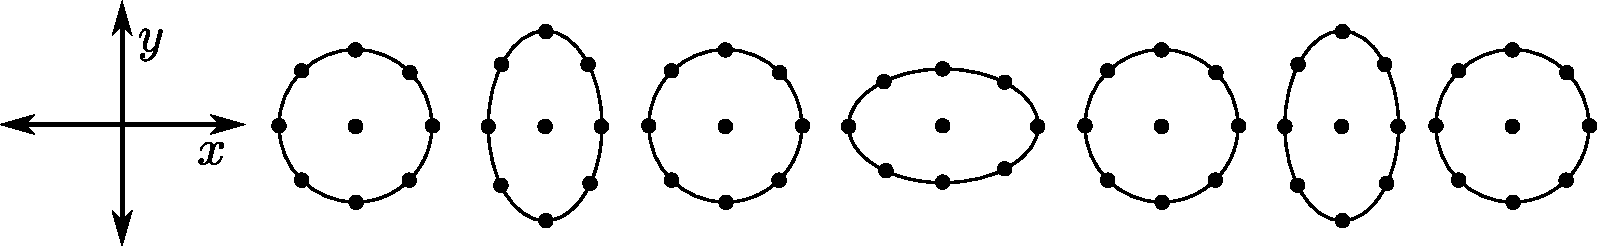
\psfig{file=fig/fig-onda-grav-mas.pdf,height=2.1cm,angle=0}}
\centerline{\psfig{file=fig/fig-onda-grav-cruz.pdf,height=2.1cm,angle=0}}
\centerline{\psfig{file=fig/fig-onda-grav-circular.pdf,height=2.1cm,angle=0}}
\caption{Oscilaciones inducidas por una onda gravitacional con polarizaci'on $+$, $\times$ y circular. Figuras adaptadas a partir de originales en \cite{Carroll97}.}
\label{fig:og}
\end{figure}
\end{center}
%\begin{center}
%\begin{figure}[H]
%\centerline{\psfig{file=fig-onda-grav-cruz.pdf,height=2.3cm,angle=0}}
%\caption{Oscilaciones inducidas por una onda gravitacional con polarizaci'on $\times$. Figura adaptada a partir de la original contenida en \cite{Carroll97}.}
%\label{fig:ogcruz}
%\end{figure}
%\end{center}
%\begin{center}
%\begin{figure}[H]
%\centerline{\psfig{file=fig-onda-grav-circular.pdf,height=2.3cm,angle=0}}
%\caption{Oscilaciones inducidas por una onda gravitacional con polarizaci'on circular. Figura adaptada a partir de la original contenida en \cite{Carroll97}.}
%\label{fig:ogccirc}
%\end{figure}
%\end{center}
Note que la amplitud del cambio de la distancia $L(\varphi)$ es $\delta L=Rh_+/2$, es decir,
\begin{equation}
\boxed{ \frac{\delta L}{L_0}\simeq h .}
\end{equation}
Se espera que los detectores de ondas gravitacionales interferom'etricos actuales alcancen una sensibilidad que permita detectar amplitudes hasta de $h\sim 10^{-20}$, que es tambi'en el orden de magnitud de la amplitud \textit{m'axima} de la radiaci'on gravitacional esperada en la Tierra debido a diversas fuentes astron'omicas. Por ejemplo, el proyecto \href{http://www.ligo.caltech.edu/}{LIGO}. consta de un interfer'ometro de 4\,km, de modo que deber'ia detectar fluctuaciones de distancia ($\delta L$) del orden de $10^{-17}\text{m}$, es decir, m'as peque\~nas que un n'ucleo at'omico!.

\begin{center}
\begin{figure}[H]
\centerline{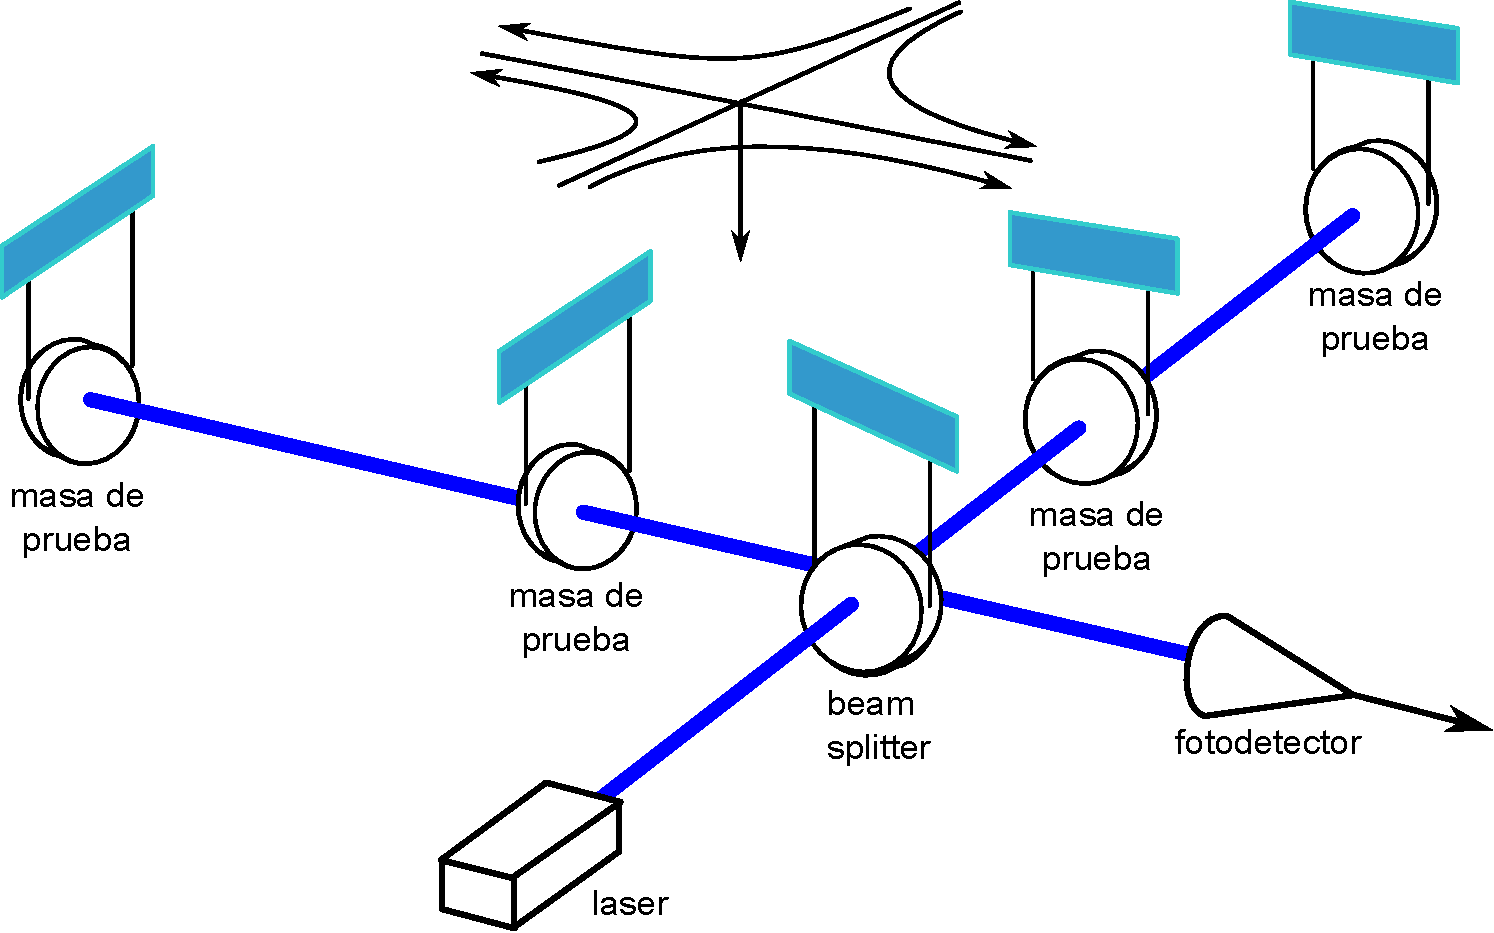
\psfig{file=fig/fig-LIGO.pdf,height=5cm,angle=0}}
\caption{Esquema de un detector interferom'etrico de ondas gravitacionales. Figura original \href{http://commons.wikimedia.org/wiki/File:Ligo.svg}{aqu'i}.}
\label{fig:LIGO}
\end{figure}
\end{center}
\section{Generaci'on de ondas gravitacionales}\label{sec:GOG}
Tal como en el caso de ondas electromagn'eticas, a distancias muy grandes (en la zona lejana o zona de radiaci'on, $r\gg\lambda$) y para fuentes peque\~nas (de tama\~no $L\ll\lambda$), encontramos que el t'ermino dominante de (\ref{solh}) es
\begin{equation}\label{hradT}
\bar{h}_{\rm rad}^{\mu\nu}(\vec{x},t)=-\frac{4G}{c^4} \frac{1}{r}\int T^{\mu\nu}_{(0)}(\vec{x}',t-\frac{r}{c})\, d^3x'.
\end{equation}
Adem'as, en una regi'on limitada del espacio, la onda puede aproximarse por una onda plana. En el gauge de Lorenz, toda la informaci'on de la onda est'a contenida en las componentes puramente espaciales $\bar{h}^{ij}$, ver (\ref{AA}). Adem'as, podemos expresar la integral (retardada) $\int T^{ij}_{(0)}\,d^3x$ en t'erminos de derivadas del momento cuadrupolar de la fuente. En efecto, usando la ley de conservaci'on para el tensor de energ'ia-momentum $T^{\mu\nu}_{(0)}$, podemos escribir
\begin{eqnarray}
 \int \partial_k(T^{ik}_{(0)}x^j)\,d^3x&=&\int (\partial_kT^{ik}_{(0)})x^j\,d^3x +\int T^{ij}_{(0)}\,d^3x \\
&=&-\int (\partial_0T^{i0}_{(0)})x^j\,d^3x +\int T^{ij}_{(0)}\,d^3x \\
&=&-\frac{1}{c}\frac{d\ }{dt}\int T^{i0}_{(0)}x^j\,d^3x +\int T^{ij}_{(0)}\,d^3x .
\end{eqnarray}
Pero la expresi'on del lado izquierdo puede transformarse en una integral de superficie en la frontera del volumen de integraci'on, que encierra la distribuci'on de energ'ia-momentum que genera el campo gravitacional. Asumiendo que esta distribuci'on est'a confinada a una regi'on acotada del espacio, tendremos que la integral de superficie se anula y por lo tanto
\begin{equation}
 \int T^{ij}_{(0)}\,d^3x =\frac{1}{c}\frac{d\ }{dt}\int T^{i0}_{(0)}x^j\,d^3x.
\end{equation}
Ya que $T^{ij}$ es sim'etrico podemos equivalentemente escribir
\begin{equation}\label{intT1}
 \int T^{ij}_{(0)}\,d^3x =\frac{1}{2c}\frac{d\ }{dt}\int \left(T^{i0}_{(0)}x^j+T^{j0}_{(0)}x^i\right)\,d^3x.
\end{equation}
Efectuamos ahora un an'alisis similar con la expresi'on $\int\partial_k(T^{0k}_{(0)}x^ix^j)\,d^3x$, que tambi'en es nula debido a que puede transformarse a una integral de superficie fuera de la regi'on con fuentes:
\begin{eqnarray}
 0&=&\int\partial_k(T^{0k}_{(0)}x^ix^j)\,d^3x\\
&=&\int(\partial_kT^{0k}_{(0)})x^ix^j\,d^3x+\int \left(T^{0i}_{(0)}x^j+T^{0j}_{(0)}x^i\right)\,d^3x\\
&=&-\int(\partial_0T^{00}_{(0)})x^ix^j\,d^3x+\int \left(T^{0i}_{(0)}x^j+T^{0j}_{(0)}x^i\right)\,d^3x\\
&=&-\frac{1}{c}\frac{d\ }{dt}\int T^{00}_{(0)}x^ix^j\,d^3x+\int \left(T^{0i}_{(0)}x^j+T^{0j}_{(0)}x^i\right)\,d^3x.
\end{eqnarray}
Por lo tanto,
\begin{equation}\label{intT2}
 \int \left(T^{0i}_{(0)}x^j+T^{0j}_{(0)}x^i\right)\,d^3x=\frac{1}{c}\frac{d\ }{dt}\int T^{00}_{(0)}x^ix^j\,d^3x.
\end{equation}
De esta forma, usando (\ref{intT1}) y (\ref{intT2}) encontramos que
\begin{equation}
 \int T^{ij}_{(0)}\,d^3x=\frac{1}{2c^2}\frac{d^2\ }{dt^2}\int T^{00}_{(0)}x^ix^j\,d^3x,
\end{equation}
y entonces
\begin{equation}
\bar{h}_{\rm rad}^{ij}(\vec{x},t)=-\frac{2G}{c^4} \frac{1}{r}\frac{d^2\ }{dt^2}\left[\frac{1}{c^2}\int T^{00}_{(0)}(x')\,x'^ix'^j\,d^3x'\right]_{\rm ret}.
\end{equation}
Como $T^{00}_{(0)}/c^2=\rho(\vec{x},t)$ es la densidad de masa de la fuente (a primer orden), se acostumbra escribir
\begin{equation}\label{hrad}
\boxed{\bar{h}_{\rm rad}^{ij}(\vec{x},t)=-\frac{2G}{c^4} \frac{1}{r}\left[\ddot{M}^{ij}\right]_{\rm ret},}
\end{equation}
donde
\begin{equation}
M^{ij}(t):=\int \rho(\vec{x},t)\,x^ix^j\,d^3x,
\end{equation}
es el \textit{tensor momento de inercia} (con traza) de la fuente.

Note que $\bar{h}_{\rm rad}^{ij}$ (b'asicamente, el potencial gravitacional de la onda generada) decae con $1/r$ y que la primera contribuci'on no nula corresponde a \textit{radiaci'on cuadrupolar}. Esta diferencia con el caso de ondas electromagn'eticas se debe a que la derivada temporal del \textit{momento dipolar gravitacional} $\int \rho x^i\,d^3x$ es proporcional al momentum lineal del sistema, que es conservado (constante) a primer orden, por lo que no aporta a la energ'ia radiada (que depende de la derivada de $\bar{h}_{\rm rad}^{ij}$).

\subsection{Ejemplo}
Consideremos un ejemplo sencillo, en el que dos cuerpos, cada uno de masa $M$, con una separaci'on $2R$, rotan con velocidad angular $\omega$ en un movimiento no-relativista en torno al centro de masa del sistema. Si modelamos las posiciones de ambas masas por $\vec{x}=\pm(R\cos(\omega t),R\sen(\omega t),0)$, es decir en el plano $xy$ y con posiciones iniciales en el eje $x$, tendremos que (la segunda derivada d)el tensor momento de inercia ser'a
\begin{equation}
 \ddot{M}^{ij}=-4MR^2\omega^2\left(
\begin{array}{ccc}
 \cos(2\omega t) & \sen(2\omega t) &0 \\
\sen(2\omega t) & -\cos(2\omega t) &0 \\
0&0&0
\end{array}\right).
\end{equation}
Con esto, (\ref{hrad}) implica que
\begin{eqnarray}
\bar{h}_{\rm rad}^{ij}(\vec{x},t)&=&\frac{8GMR^2\omega^2}{c^4r}\left(
\begin{array}{ccc}
 \cos\left[2\omega(t-r/c)\right] & \sen\left[2\omega(t-r/c)\right] &0\\
\sen\left[2\omega(t-r/c)\right] & -\cos\left[2\omega(t-r/c)\right] &0\\
0&0&0
\end{array}\right)\\
&=&\frac{8GMR^2\omega^2}{c^4r}\left[
\left(\begin{array}{ccc} 1 & 0 & 0\\ 0 & -1 &0 \\ 0&0&0\end{array}\right) \cos\left[2\omega(t-r/c)\right]
+\left(\begin{array}{ccc} 0 & 1 &0 \\ 1 & 0&0\\ 0&0&0\end{array}\right) \sen\left[2\omega(t-r/c)\right]
\right] \nonumber\\
&=&\frac{8GMR^2\omega^2}{c^4r}\Re\left[
\left(\begin{array}{ccc} 1 & 0 &0 \\ 0 & -1 &0 \\ 0&0&0\end{array}\right) e^{i\left[2\omega(t-\frac{r}{c})\right]} +\left(\begin{array}{ccc} 0 & 1 &0 \\ 1 & 0 &0 \\ 0&0&0\end{array}\right) e^{i\left[2\omega(t-\frac{r}{c})-\frac{\pi}{2}\right]}
\right] .
\end{eqnarray}
Vemos de aqu'i que \textit{un observador ubicado en un punto sobre el eje} $z$ detectar'a una onda gravitacional de frecuencia angular $2\omega$, que \textit{satisface autom'aticamente el gauge TT}, y que es una combinaci'on lineal de las polarizaciones $+$ y $\times$, con una diferencia de fase de $\pi/2$. Este estado es an'alogo al de una onda electromagn'etica con polarizaci'on circular.

El orden de magnitud de la amplitud de la onda es dada por
\begin{equation}
 h\simeq\frac{8GMR^2\omega^2}{c^4r}=8\left( \frac{GM}{c^2}\right) \left( \frac{1}{r}\right) \left( \frac{\omega R}{c}\right)^2 =8\left( \frac{m}{r}\right) \left( \frac{v}{c}\right) ^2.
\end{equation}
Por ejemplo, el pulsar binario PSR 1913+16 consta de 2 estrellas de neutrones de masa $M\approx 1.4 M_\odot$, con periodo orbital $T\approx 8\text{\,h}\approx 3\times 10^4\text{\,s}$, velocidades orbitales $v\simeq 10^2\text{\,km/s}$, a una distancia $r\approx 2\times 10^4\text{\, ly}\approx 10^{20}\text{\, m}$. En este caso, $m\approx 2\text{\,km}$, $v/c\simeq 3\times 10^{-4}$ y entonces $h\simeq 10^{-23}$ para la radiaci'on recibida en la Tierra, a una frecuencia del orden de $10^{-4}Hz$ (no detectable con LIGO).




